%%% Local Variables:
%%% TeX-command-extra-options: "-shell-escape"
%%% mode: latex
%%% TeX-master: t
%%% End:
\documentclass{beamer}
\usepackage{caption}
\usepackage{minted}
\usepackage{tikz}
\usepackage{xcolor}
\usetikzlibrary{shapes.geometric, arrows}
\tikzstyle{startstop} = [rectangle, rounded corners, minimum width=3cm, minimum height=1cm,text centered, draw=black, fill=red!30]
\tikzstyle{io} = [trapezium, trapezium left angle=70, trapezium right angle=110, minimum width=1.5cm, minimum height=0.6cm, text centered, draw=black, fill=blue!30]
\tikzstyle{process} = [rectangle, minimum width=1.5cm, minimum height=0.5cm, text centered, draw=black, fill=orange!30]
\tikzstyle{decision} = [circle, radius=2.5cm, text centered, draw=black, fill=green!30]
\tikzstyle{arrow} = [thick,->,>=stealth]
\usepackage[labelformat=simple]{subcaption}

\usetheme{Singapore}
\title{Structures and All That}
\begin{document}
\begin{frame}
\titlepage
\end{frame}
\section{Compound Data}

\begin{frame}
``Here at Brymar College\\
We can get you prepared for the 31st century\\
With advanced programming and quad rendering\\
And Java plus plus plus scripting language\\
We offer advanced job placement assistance''\\\\
from Upgrade by Deltron 3030  
\end{frame}

\begin{frame}
  \frametitle{Data Descriptions Matter}
  We have taken a weird approach by fixating on data structured in the form of ``or'' first.
  \begin{itemize}
  \item<2-> We would say that a traffic light's state is red \textbf{\emph{or}} yellow \textbf{\emph{or}} green. I will sometimes refer to data
    in this form as defining a \emph{sum type}, but for now I will stick to saying itemization.
  \item<3-> But tons of data is written in a compound manner. A person has a head \textbf{\emph{and}} a face \textbf{\emph{and}} a body ...
    I will sometimes refer to data in this form as being a \emph{product type}, but will usually stick to saying \emph{struct}.
    When I talk about classes, I will be talking about more than compound data.
  \item<4-> Whereas with ``or'' we would check which kind of data we would have and then use a computation specific to that data, with
    products we can directly project out data.
  \item<5-> Let's say that in Java that you have some person class with a first and last name represented as strings.
  \item<6-> It is easy to define a method that returns the person's full name by concatenating the first and last name.
  \end{itemize}
\end{frame}



\begin{frame}
  \frametitle{Who Needs Structs Anyway?}
  So, why do we need compound data?
  \begin{itemize}
  \item<2-> The obvious answer is that we have programs that have some kind of compound state.
  \item<3-> Consider the simple program where we wanted to move a dot left and right.
  \item<4-> We were able to represent the state of the world as a single position number.
  \item<5-> Let's add another dimension of movement where we can now move the dot up and down.
  \item<6-> Can we represent the state of the world as a single number?
  \item<7-> If you said no, I get it! But that happens to be incorrect.
  \item<8-> We can represent a grid  with one number in the same sense that we can simulate a 10x10 2D array
    with a 100 element array.
  \end{itemize}
\end{frame}

\begin{frame}
  \frametitle{Structs Make Things Easier}
  Personally, I like doing things the easy way.
  \begin{center}
    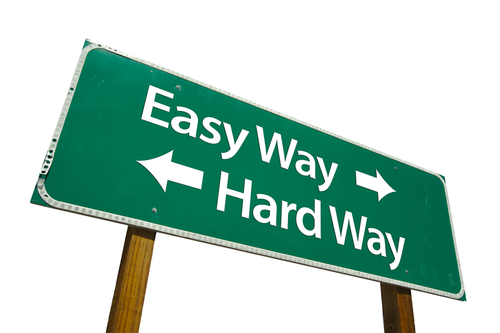
\includegraphics{images/easy-way.jpg}
  \end{center}  
\end{frame}

\defverbatim[colored]\fstName{
\begin{minted}{python}
def first_name(tup):
  return tup[0]
\end{minted}
}

\begin{frame}
  \frametitle{Unstructured Compound Data?}
  We can actually represent compound data without needing to provide names for the individual pieces of data.
  \begin{itemize}
  \item<2-> Let's consider some individual examples in Python.
  \item<3-> We can represent a Person with a first name, last name, and age with the following kind of tuple:
  \item<4-> \mintinline{python}{("Peter", "Campora", 26)}
  \item<5-> We could then define functions to act like field accesses.
  \item<6-> \fstName
  \end{itemize}
\end{frame}

\begin{frame}
  \frametitle{Data (Un)Structures}
  We can actually define other data structures in terms of things like lists.
  \begin{itemize}
  \item<2-> Let's consider defining a binary tree in terms of a python list.
  \item<3-> We can define a null node with \mintinline{python}{[]}
  \item<4-> A tree with a single root element can be \mintinline{python}{[[] 1 []]}
  \item<5-> Here's a nice balanced tree \mintinline{python}{[[[] 1 []] 2 [[] 3 []]]}
  \item<6-> This representation gets a bit ugly fast, huh?
  \item<7-> So Python gives classes (or named tuples) as a way to more easily
    define such structured data.
  \end{itemize}
\end{frame}

\begin{frame}
  \frametitle{Unstructured Data in Racket}
  Similarly, we can define data using pairs and lists in Racket.
  \begin{itemize}
  \item<2-> We can write a pair $(1, 2)$ as \mintinline{racket}{(1 . 2)}.
  \item<3-> We can write a linked list 1$\rightarrow$2-$\rightarrow$3$\rightarrow$4$\rightarrow$empty as \mintinline{racket}{'(1 2 3 4)}
  \item<4-> To get the first element in the linked list, you can write:
    \mintinline{racket}{(first '(1 2 3 4))}$\hookrightarrow$ \mintinline{racket}{1}
  \item<5-> To get the rest of the linked list you can write
    \mintinline{racket}{(rest '(1 2 3 4))}$\hookrightarrow$ \mintinline{racket}{'(2 3 4)}
  \item<6-> The empty list is represented with \mintinline{racket}{'()}
    and you can check for the empty list with \mintinline{racket}{(empty? '())}
    $\hookrightarrow$ \mintinline{racket}{\#t}
  \item<7-> We will return to discussing lists in more detail later,
    since they are \emph{extremely} important.
  \item<8-> But for now, remember that we wanted to avoid the inconveniences
    given by using other existing data types to represent some piece of compound data!
  \end{itemize}
\end{frame}

\begin{frame}
  \frametitle{The Talk}
  We said that we didn't want to represent all of our compound data with
  existing structures like lists are tuples, so
  let's \emph{finally} talk about structs.
  \begin{itemize}
  \item<2-> Let's reconsider our 2 dimensional movement program.
  \item<3-> We need a natural representation for cartesian coordiantes for the state of our world.
  \item<4-> We could obviously have the state of our our world be a pair
    \mintinline{racket}{'(x . y)} or a list \mintinline{racket}{'(x  y)}
  \item<5-> But it would be better if we had piece of compound data with two fields, one field named x to represent the x coordinate and similarly a y...
  \item<6-> To define the struct: \mintinline{racket}{(struct point [x y])}
  \item<7-> To make a new point: \mintinline{racket}{(define one-two (point 1 2))}
  \item<8-> To get the x-coordinate: \mintinline{racket}{(point-x one-two)}
  \end{itemize}
\end{frame}

\defverbatim[colored]\distance{
\begin{minted}{racket}
    ;;Point -> Number
    ;;Compute a point's distance from the origin
    (define (distance-to-0 ap) 0)
\end{minted}
}

\defverbatim[colored]\distanceExamples{
\begin{minted}{racket}
    (check-expect (distance-to-0 (point 0 5)) 5)
    (check-expect (distance-to-0 (point 7 0)) 7)
\end{minted}
}

\defverbatim[colored]\distanceSkeleton{
\begin{minted}{racket}
    (define (distance-to-0 ap)
      (... (point-x ap) ...
       ... (point-y ap) ...))
\end{minted}
}

\defverbatim[colored]\distanceFinal{
\begin{minted}{racket}
    (define (distance-to-0 ap)
      (sqrt
        (+ (sqr (point-x ap))
           (sqr (point-y ap)))))
\end{minted}
}

\begin{frame}
  \frametitle{Writing Simple Programs With Structs}
  Before we consider writing more complex applications involving structs,
  let's consider writing a simple function.
  \begin{itemize}
  \item<2-> Let's consider computing the distance to the origin where we
    take in one parameter that is a point, instead of taking two parameters
    for an x-coordinate and y-coordinate.
  \item<3-> As will happen many times in this course, we will introduce
    the concept by examples before we cover how our design recipes change
    to address this new feature
  \item<4-> \distance
  \item<5->Let's add functional examples as tests:
  \item<6-> \distanceExamples
  \end{itemize}
\end{frame}

\begin{frame}
  \frametitle{Structs and Skeletons}
  We now can take inventory (step 4) and add a skeleton for our function.
  In this case we should know that we have to project out the x-coordinate
  and the y-coordinate in our distance function.
  \begin{itemize}
  \item<2-> \distanceSkeleton
  \item<3-> To code, we essentially have the same logic as when we had a previous
    version of this function that took in two parameters. Now, we just use
    the projected out x-coordinate and y-coordinate from our point.
  \item<4-> \distanceFinal
  \end{itemize}
\end{frame}

\begin{frame}
  \frametitle{Structs in General}
  Testing that function is simple, so let's just move on to talking about
  structs in general.
  \begin{itemize}
  \item<2-> You can define a struct in general with:
    \mintinline{racket}{(struct s-name [field-name-1 ...field-name-n])}
  \item<3-> After creating a struct, 3 kinds of functions are automatically
    made for you.
    \begin{enumerate}
    \item<4-> One constructor, a function that creates structure instances. It takes as many values as there are fields; as mentioned, structure is short for structure instance. The phrase structure type is a generic name for the collection of all possible instances;
    \item<5-> One selector per field, which extracts the value of the field from a structure instance; and
    \item<6-> One structure predicate, which, like ordinary predicates, distinguishes instances from all other kinds of values.
    \end{enumerate}
  \end{itemize}
\end{frame}

\begin{frame}
  \frametitle{Basic Struct Options}
  Let's illustrate each of these three kinds of functions, with our point
  struct.
  \begin{enumerate}
  \item<2-> The constructor is: \mintinline{racket}{(point x-val y-val)}
    where x-val and y-val will be values passed to the x-field and y-field in
    our point struct. The general form is \mintinline{racket}{(struct-name field-name-1-arg ... field-name-n-arg)}
  \item<3-> The selectors per field are \mintinline{racket}{(point-x point-val)} and \mintinline{racket}{(point-y point-val)}. The general form
    of a selector for a specific field is \mintinline{racket}{(struct-name-field-name val)}
  \item<4-> A predicate for checking types is automatically created, for example:
    \mintinline{racket}{(point? point-val)} and in general a predicate
    \mintinline{racket}{struct?} is created.
  \end{enumerate}
\end{frame}

\begin{frame}
  \frametitle{Examples of Structs}
  Here are some basic examples of structs:
  \begin{itemize}
  \item<2-> \mintinline{racket}{(struct movie [title producer year])}
  \item<3-> \mintinline{racket}{(struct person [name hair eyes phone])}
  \item<4-> You guys should be able to think of many more examples.
    \item<5-> \textbf{Sample Problem} Develop a structure type definition for a program that deals with “bouncing balls,”. The ball’s location is a single number, namely the distance of pixels from the top. Its constant speed is the number of pixels it moves per clock tick. Its velocity is the speed plus the direction in which it moves.
  \end{itemize}
  
  
\end{frame}

\begin{frame}
  \frametitle{Designing Our Ball Struct}
  Since we are talking about a ball that bounces up and down, our structure definition is pretty simple. We need a single number for the y position and single
  number for the velocity in the y-axis.
  \begin{itemize}
  \item<2-> \mintinline{racket}{(struct ball [location vec])}
  \item<3-> This is simple because our ball is moving in a single direction. But if we had a Brick Breaker esque game then we would have a bouncing ball that
    travels along a 2D plane, then our definition is much more complicated.
  \item<4-> Let's first consider defining a 2D vector struct as follows: \mintinline{racket}{(struct vector [delta-x delta-y])}
  \item<5-> Now, we can represent a ball as a point (which only has positive components) and a vector (which can have negative components):
    \mintinline{racket}{(struct 2D-ball position vec)}
  \end{itemize}
\end{frame}

\defverbatim[colored]\pointDefinition{
\begin{minted}[fontsize=\footnotesize]{racket}
    (define-struct point [x y])
    ; A Point is a structure: 
    ;   (point Number Number)
    ; interpretation a point x pixels from left, y from top
\end{minted}
}

\begin{frame}
  \frametitle{Other Representations}
  Our 2D Ball struct has nested occurrences of other structs. This is a natural thing, and even recursive descriptions of data are natural, i.e.
  linked lists and binary trees. But we can also consider using a \emph{flat representation} for our 2D Ball, which doesn't nest structs.
  \begin{itemize}
  \item<2-> \mintinline{racket}{(struct 2D-ball [x y delta-x delta-y]}
  \item<3-> Although valid, I think it's better to keep representations natural and just nest things, barring performance concerns.
  \item<4-> Let's talk about defining data definitions for structs. We must specify the form of the struct and the types of its field and provide an interpretation of what
    each of the fields represents. Here's how we do this for our point struct:
  \item<5->\pointDefinition
  \end{itemize}
\end{frame}

\defverbatim[colored]\moveDotStart{
\begin{minted}{racket}
(define MTS (empty-scene 100 100))
(define DOT (circle 3 "solid" "red"))
 
; A Point represents the state of the world.
 
; Point -> Point
(define (main p0)
  (big-bang p0
    [on-tick x+]
    [on-mouse reset-dot]
    [to-draw scene+dot]))   
\end{minted}
}

\begin{frame}
  \frametitle{Computing With Structures}
  As mentioned, we could have use tuples instead of structs to represent
  compound data, but remembering to access the name field of a person
  struct is a lot easier than remembering to project out the 7th element
  in some n-tuple (assuming n>=7).
  \begin{itemize}
  \item<2-> How does \emph{computing} with structures become more natural than simply computing with tuples?  
  \item<3-> We can provide  a natural data representation that simplifies the coding process by giving us easy to remember
    field-names to select.
  \item<4-> Let us consider how to relate a struct description
    to a diagram that illustrates its ``structure''.
  \item<5-> \mintinline{racket}{(struct centry [name home office cell])}
  \end{itemize}
\end{frame}

\begin{frame}
  \frametitle{Struct Structure}
  So, for cell phone entry structs we had three fields that can contain
  possible values. Consider the following concrete one:
  \begin{itemize}
  \item<2->
    \mintinline[fontsize=\footnotesize]{racket}{(define pl (centry "Al Abe" "666-7771" "lee@x.me"))}
  \item<3-> This has the following visual representation:
    \includegraphics[width=0.3\textwidth]{images/cell-struct.png}
  \item<4-> In a sense, calling \mintinline{racket}{(centry-name pl)} is unlocking a box in the struct, with a specific key that
    allows you to retrieve the underlying value. In general we can
    think of field access as a kind of ``unboxing''.
  \item<5-> Using a ``key'' to unlock the wrong box raises a runtime
    error \mintinline{racket}{(centry-name (point 1 2))}$\hookrightarrow$ \textcolor{red}{entry-name:expects a centry, given (point 42 5)}    
  \end{itemize}
\end{frame}

\begin{frame}
  \frametitle{Some Definitions}
  \begin{itemize}
  \item \textbf{Syntax} - the arrangement of words and phrases to create well-formed sentences in a language.
  \item<2-> \textbf{Semantics} - the branch of linguistics and logic concerned with meaning. There are a number of branches and subbranches of semantics, including formal semantics, which studies the logical aspects of meaning, such as sense, reference, implication, and logical form, lexical semantics, which studies word meanings and word relations, and conceptual semantics, which studies the cognitive structure of meaning.
  \item<3-> \textbf{Interpretation} - the action of explaining the meaning of something.
  \item<4-> \textbf{Denotation} - the object or concept to which a term refers, or the set of objects of which a predicate is true.
  %\item<4-> \textbf{Polymorphism} - the condition of occurring in several different forms.
  \end{itemize}  
\end{frame}

\begin{frame}
  \frametitle{A Few More}
  \begin{itemize}
  \item \textbf{Compiler} - a computer program that translates computer code written in one programming language (the source language) into another language (the target language).
  \item<2-> \textbf{Computable Function} - A function that can be represented by a \emph{general recursive function}, a \textbf{lambda computable function}, or
    a \textbf{Turing Machine}
  \item<3-> \textbf{Programming Language} - a formal language, which comprises a set of instructions that produce various kinds of output. Programming languages are used in computer programming to implement algorithms.
  \item<4->  I kind of dislike this definition.
  \item<5-> My definition - A formal language that has a computable semantics specifying the denotation of a ``sentence'' written in the language. This denotation  can be given by compilation into some other formal language, or by a direct interpretation.
  \end{itemize}
\end{frame}

\begin{frame}
  \frametitle{Some Important People}
  \begin{center}
    \includegraphics[width=0.7\textwidth]{images/godel-turing-church.png}\\
    \pause
    \includegraphics[width=0.2\textwidth]{images/carl-jung.jpeg}
  \end{center}
\end{frame}

\begin{frame}
  \frametitle{Natural Interpretations?}
  Here's a fun little experiment. Look at these two shapes:
  \begin{center}
    \includegraphics[width=0.7\textwidth]{images/bouba-kiki.png}
  \end{center}
  \begin{itemize}
  \item<2-> Which of these shapes is named Bouba and which Kiki?
  \item<3-> This is likely due to some physical attributes of sound, but
    our strong preference for naming the round one Bouba and the
    sharp one Kiki shows that humans have \textbf{innate preferences}
    about the \emph{naming} and \emph{representation of things}.
  \end{itemize}
\end{frame}

\defverbatim[colored]\BallInterp{
\begin{minted}{racket}
    (define-struct ball [location velocity])
    ; A Ball-1d is a structure:  
    ;   (ball Number Number)
    ; interpretation 1 distance to top and velocity 
    ; interpretation 2 distance to left and velocity 
\end{minted}
}

\begin{frame}
  \frametitle{Interpreting Structure}
  In general, we need to think about how we describe the
  interpretation of structs.
  \begin{itemize}
  \item<2-> Defining a data interpretation for the ball with one dimensional  movement is simple. We can describe position and the
    velocity in terms of numbers.
  \item<3-> \BallInterp
  \item<4-> Interestingly, we can give 2 interpretations, depending
    on if the ball is moving vertically (interpretation 1) or
    horizontally (interpretation 2)
  \end{itemize}
\end{frame}

\defverbatim[colored]\NestedInterp{
\begin{minted}{racket}
    ; A Ball-2d is a structure: 
    ;   (ball Point Vel)
    ; interpretation a 2-dimensional position and velocity
 
    (define-struct vel [deltax deltay])
    ; A Vel is a structure: 
    ;   (vel Number Number)
    ; interpretation (make-vel dx dy) means a velocity of 
    ; dx pixels [per tick] along the horizontal and
    ; dy pixels [per tick] along the vertical direction
\end{minted}
}

\begin{frame}
  \frametitle{Interpreting Structure (cont.)}
  Interpretations become slightly more interesting with nested
  structures.
  \begin{itemize}
  \item<2-> Consider the ball that can move in two dimensions.
  \item<3-> Since the ball relies on a vector struct, it is important
    to make sure that the vector also has an interpretation.
  \item<4-> \NestedInterp
  \end{itemize}
\end{frame}

\defverbatim[colored]\LinkedListInterp{
\begin{minted}{racket}
    ; A LinkedList is a structure:
    ; (linked-list T LinkedList)
    ; interpretation a value contained in the current node
    ; and a reference to the rest of the list
\end{minted}
}

\begin{frame}
  \frametitle{Interpreting Structure (cont.)}
  Recursively defined types don't add any problems
  to writing data interpretations.
  \begin{itemize}
  \item<2-> What are some famous recursively defined types?
  \item<3-> Let's consider a linked list.
  \item<4-> \LinkedListInterp
  \item<5-> We don't have to worry about the recursive instance of
    the type, since we are currently interpreting it.
  \item<6-> The T just communicates that we are defining linked lists
    that work over any type (\emph{parametric polymorphism} otherwise
    known as \emph{generics} in Java)
  \end{itemize}
\end{frame}


\begin{frame}
  \frametitle{Structs and Program Design}
  Now we need to consider designing programs using structs.
  \textbf{Sample Problem} Your team is designing an interactive game program that moves a red dot across a image canvas and allows players to use the mouse to reset the dot. Here is how far you got together: \pause
  \moveDotStart
\end{frame}

\defverbatim[colored]\sceneDotHeader{
\begin{minted}{racket}
    ; Point -> Image
    ; adds a red spot to MTS at p
    (define (scene+dot p) MTS)
\end{minted}
}

\defverbatim[colored]\sceneDotExamples{
\begin{minted}{racket}
    (check-expect (scene+dot (point 10 20))
                  (place-image DOT 10 20 MTS))
    (check-expect (scene+dot (point 88 73))
                  (place-image DOT 88 73 MTS))

\end{minted}
}

\defverbatim[colored]\sceneDotSkeleton{
\begin{minted}{racket}
    (define (scene+dot p)
      (... (point-x p) ... (point-y p) ...))
\end{minted}
}

\begin{frame}
  \frametitle{Designing scene+dot}
  Let us first assume that you're tasked with designing \mintinline{racket}{scene+dot}.
  \begin{itemize}
  \item<2-> Of course, we already have our data interpretation so we start
    with step 2 and provide our signature, statement of purpose, and
    function header.
  \item<3-> \sceneDotHeader
  \item<4-> Finishing step 3 and creating the following functional examples (as tests) is straightforward:
  \item<5-> \sceneDotExamples
  \end{itemize}
\end{frame}

\defverbatim[colored]\sceneDotFinal{
\begin{minted}{racket}
    (define (scene+dot p)
      (place-image DOT (point-x p) (point-y p) MTS))
\end{minted}
}

\begin{frame}
  \frametitle{Designing scene+dot (cont.)}
  We can now move on to carrying out step 4 and taking inventory:
  \begin{itemize}
  \item<2-> \sceneDotSkeleton
  \item<3-> Finishing step 5 is easy, we simply need to place the
    projected x and y coordinates as arguments to \mintinline{racket}{place-image}
  \item<4-> \sceneDotFinal
  \item<5-> Testing this is uninteresting, so let's consider if we were asked
    to define the \mintinline{racket}{x+} function, which takes in a Point
    and returns a new Point with an x-coordinate that is 3 units further to
    the right of the old point.    
  \end{itemize}
\end{frame}

\defverbatim[colored]\xPlusHeader{
\begin{minted}{racket}
    ;;Point -> Point
    ;;Updates the position of our dot at each clock tick
    (define (x+ p) p)
\end{minted}
}

\defverbatim[colored]\xPlusExamples{
\begin{minted}{racket}
    (check-expect (x+ (point 0 0)) (point 3 0))
    (check-expect (x+ (point 10 10)) (point 13 10))
    (check-expect (x+ (point 0 10)) (point 3 10))
\end{minted}
}

\defverbatim[colored]\xPlusSkeleton{
\begin{minted}{racket}
    (define (x+ p) (... (point-x p) ... (point-y p) ...)
\end{minted}
}

\begin{frame}
  \frametitle{Designing x+}
  Designing our  \mintinline{racket}{x+} function is a bit harder than
  \mintinline{racket}{scene+dot}, because we are producing structures
  as output.
  \begin{itemize}
  \item<2-> When carrying out step 2, recall that \mintinline{racket}{x+} handles clock ticks:
    \xPlusHeader
  \item<3-> Coming up with functional examples as tests is
    straightforward:
    \xPlusExamples
  \item<4-> To take inventory we project out the x and y fields
    from our point, as usual:
    \xPlusSkeleton
  \end{itemize}
\end{frame}

\defverbatim[colored]\xPlusFinal{
\begin{minted}{racket}
    (define (x+ p)
      (point (+ (point-x p) 3) (point-y p)))
\end{minted}
}

\begin{frame}
  \frametitle{Designing x+ (cont.)}
 To finish coding, we need to first add 3 to the x-coordinate
 and then pack the result back into a new point structure.
 \begin{itemize}
 \item<2-> \xPlusFinal
 \item<3-> This is a perfect example of the \emph{essence} of
   functional programming. We are creating a \emph{new} point
   whose x-coordinate is based on the old one, instead of modifying
   the original point to store a new x-coordinate.
 \item<4-> But there is something inelegant about this, right?
 \item<5-> If we had more fields than y, we simply are projecting
   out the old field as an argument when creating the new struct
   value.
 \item<6-> This adds a lot of boilerplate code...
 \end{itemize}
\end{frame}

\defverbatim[colored]\pointSet{
\begin{minted}{racket}
    (define (point-set-x p x)
      (point x (point-y p))
\end{minted}
}

\defverbatim[colored]\xPlusNew{
\begin{minted}{racket}
    (define (x+ p)
      (point-set-x p (+ (point-x p) 3)))
\end{minted}
}

\begin{frame}
  \frametitle{Struct Boilerplate}
  We might want to define a function, \mintinline{racket}{point-set-x} which takes in a point and a value
  and produces a new point where the x-coordinate is the given value and the y-coordinate is taken from the old point.
  \begin{itemize}
  \item<2-> Here is the code: \pointSet
  \item<3-> We can now redefine \mintinline{racket}{x+} with it:
    \xPlusNew
  \item<4-> \mintinline{racket}{point-set-x} is  known as
    a \emph{functional setter}, similar to a more traditional setter
    in languages like Java.
  \item<5-> However, defining an update operation on a complicated
    structure can get very complicated, and we can get around
    this uses \emph{lenses} (we may discuss this later in the course).
  \end{itemize}  
\end{frame}

\defverbatim[colored]\ResetDotHeader{
\begin{minted}{racket}
    ; Point Number Number MouseEvt -> Point 
    ; for mouse clicks, (point x y); otherwise p
    (define (reset-dot p x y me) p)
\end{minted}
}

\defverbatim[colored]\ResetDotExamples{
\begin{minted}{racket}
    (check-expect
      (reset-dot (point 10 20) 29 31 "button-down")
      (point 29 31))
    (check-expect
      (reset-dot (point 10 20) 29 31 "button-up")
      (point 10 20))
\end{minted}
}

\defverbatim[colored]\ResetDotSkeleton{
\begin{minted}{racket}
    (define (reset-dot p x y me)
      (cond
        [(mouse=? "button-down" me) (... p ... x y ...)]
        [else (... p ... x y ...)]))
\end{minted}
}

\defverbatim[colored]\ResetDotFinal{
\begin{minted}{racket}
    (define (reset-dot p x y me)
      (cond
        [(mouse=? me "button-down") (point x y)]
        [else p]))
\end{minted}
}

\begin{frame}
  \frametitle{Events Creating Structs}
  We can consider designing a function \mintinline{racket}{reset-dot}
  which places a dot where a mouse is clicked.
  \begin{itemize}
  \item<2-> We start with step 2 and create a signature, statement of
    purpose, and stub for this function.
  \item<3-> \ResetDotHeader
  \item<4-> The statement of purpose and the signature should make
    designing the functional examples easy.
  \item<5-> \ResetDotExamples
  \end{itemize}
\end{frame}

\begin{frame}
  \frametitle{Events Creating Structs (cont.)}
  From here, writing the skeleton and finishing coding are easy.
  \begin{itemize}
  \item<2-> The Skeleton:    
    \includegraphics[width=0.4\textwidth]{images/skeletor.jpeg}
  \item<3-> For real this time:    \ResetDotSkeleton
  \end{itemize}
\end{frame}

\begin{frame}
  \frametitle{Events Creating Structs (cont.)}
      Finally, though the skeleton looks complicated the final version
    of the function is relatively simple.
  \begin{itemize}
  \item<2-> \ResetDotFinal
  \item<3-> The takeaway here is that our skeletons can end up being
    more complicated than the actual final version.
  \item<4-> This is especially true when we consider skeletoning
    out code for which a parameter is a struct.
  \end{itemize}
\end{frame}

\defverbatim[colored]\ComplexSkeleton{
\begin{minted}{racket}
    (define (complex-skeleton ball)
      (... (point-x (ball-position ball)) ...
       ... (point-y (ball-position ball)) ...
       ... (vec-delta-x (ball-vector ball)) ...
       ... (vec-delta-y (ball-vector ball)) ...))
\end{minted}
}

\defverbatim[colored]\SimplerSkeleton{
\begin{minted}{racket}
    (define (complex-skeleton ball)
      (... (point-x (ball-position ball)) ...
       ... (vec-delta-y (ball-vector ball)) ...))
\end{minted}
}

\begin{frame}
  \frametitle{Complex Skeletons}
 Consider a skeleton for a function whose input
 is a ball moving two dimensionally.
 \begin{itemize}
 \item<2-> We would have to write a field access for both of the
   underlying point structure's fields, along with field accesses for the underlying vector structure's fields. 
 \item<3-> It would look like the following:
   \ComplexSkeleton
 \item<4-> For some of the classes you see in Java, skeletoning
   out code in such a manner is infeasible...   
 \end{itemize}  
\end{frame}

\begin{frame}
  \frametitle{So, What's a Feasible Way?}
  So, how should we skeleton out functions with complex structs
  as input?
  \begin{itemize}
  \item<2-> \textbf{If a function deals with nested structures, develop one function per level of nesting.}
  \item<3-> For our previous example, we could have wrote:
    \SimplerSkeleton
  \item<4-> Of course, things are easier if we picked the write functions to add in our skeleton, but this keeps the structure of
    the skeleton much simpler.
  \item<5-> We will return to this point later in the course.    
  \end{itemize}   
\end{frame}

\begin{frame}
  \frametitle{A Digression About Signatures}
  Signatures can tell us a lot about a function. I'll put
  some signatures up, and what kind of functions could we write
  for these signatures?
  \begin{itemize}
  \item<1-> Number Number $\rightarrow$ Number
  \item<2-> Point Vec $\rightarrow$ Point
  \item<3-> Point $\rightarrow$ Number
  \item<4-> Vec $\rightarrow$ Number
  \item<5-> T LinkedList $\rightarrow$ LinkedList
  \item<6-> T $\rightarrow$ T
  \item<7-> The idea that a function signature can tell you
    about the behavior of the function is an extremely powerful idea.
  \end{itemize}
\end{frame}



\defverbatim[colored]\BSData{
\begin{minted}{racket}
    ; A BS is one of: 
    ; — "hello",
    ; — "world", or
    ; — pi.
\end{minted}n
}

\begin{frame}
  \frametitle{Racket Data and the Universe}
  Racket chose certain extremely powerful data types as primitives
  that make up our initial \emph{data universe}.
  \begin{itemize}
  \item<2-> From here, we talked about enumerations, intervals,
    and itemizations as a way to restrict the kind of values from
    the universe that we want our function to consider.
  \item<3-> For example, look at this data definition:
    \BSData
  \item<4-> If this is the domain of some function, we restricted
    ourselves to needing to handle three values.  
  \end{itemize}
\end{frame}

\begin{frame}
  \frametitle{Expanding the Universe}
With itemizations we specified subsets of the existing data universe.
\begin{itemize}
  \item<1-> \includegraphics[width=0.2\textwidth]{images/BS-universe.png}    
  \item<2-> When we added structs, we actually provided the ability to
  extend the universe of data.
  \item<3-> We provided new data types describing points, balls, etc.
  \item<4-> \includegraphics[width=0.45\textwidth]{images/struct-universe.png}
  \end{itemize}
\end{frame}

\begin{frame}
  \frametitle{Respect Interpretations}
  Notice that we specify our point struct as containing
  two numbers.
  \begin{itemize}
  \item<2-> But when we added this struct, we really created a pair
    that could contain \emph{any} two values.
  \item<3-> Racket doesn't inherently stop us from writing:
    \mintinline{racket}{(point "foo" "bar")}.
  \item<4-> Typed Racket can add the exact kind of point to the universe we want and stop invalid data from being added to a point's
    field at compile time.
  \item<5-> Without that, it is up to us programmers to validate
    that points are only constructed with valid arguments.
  \item<6-> This might mean creating a function \mintinline{racket}{(define (make-point x y) ...)} that checks
    that both \mintinline{racket}{x} and \mintinline{racket}{y} actually receive integers before calling the \mintinline{racket}{point} constructor. More on this later.
  \end{itemize}
\end{frame}

\begin{frame}
  \frametitle{Respect Interpretations (cont.)}
  Data definitions are a critical part of programming.
  \begin{itemize}
  \item<2-> In Java
    when you define a class, you are saying that this class is an example
    of data that was important enough to need modeling. Making a data definition specifies that this kind of data is integral to understanding the program.  
  \item<3-> So, when adding a definition provide an example of realistic
    data for what is being defined:
  \item<4-> For a built-in collection of data (number, string, Boolean, images), choose your favorite examples. (E.G. 1)
  \item<5-> For an enumeration, use several of the items of the enumeration. (For NorF use \#f)
  \item<6-> For intervals, use the end points (if they are included) and at least one interior point.
  \item<7-> For itemizations, deal with each part separately
  \item<8-> For data definitions for structures, follow the natural language description; that is, use the constructor and pick an example from the data collection named for each field.
  \end{itemize}
\end{frame}

\begin{frame}
  \frametitle{Back to the Drawing Board}
  As usual, introducing structs necessitates that we change our design process so that we have clear
  instructions on how to deal with structs as the input and output to/of functions. We will
  illustrate the changes with the following problem:
  \begin{itemize}
  \item<2-> \textbf{Sample Problem} Design a function that computes the distance of objects in a 3-dimensional space to the origin.
  \item<3-> The first step to our design process has a bigger change than was typical for previous revisions to our design process.
  \end{itemize}
\end{frame}

\begin{frame}
  \frametitle{Step 1 and Structs}
  \begin{itemize}
  \item<2-> (1) When a problem calls for the representation of pieces of information that belong together or describe a natural whole, you need a structure type definition. It requires as many fields as there are relevant properties. An instance of this structure type corresponds to the whole, and the values in the fields correspond to its attributes.
  \item<3-> (1) A data definition for a structure type introduces a name for the collection of instances that are legitimate. Furthermore, it must describe which kind of data goes with which field. Use only names of built-in data collections or previously defined data definitions.
  \item<3-> (1) In the end, we (and others) must be able to use the data definition to create sample structure instances. Otherwise, something is wrong with our data definition. To ensure that we can create instances, our data definitions should come with data examples.
  \end{itemize}
\end{frame}

\defverbatim[colored]\stepOneStructs{
\begin{minted}[fontsize=\footnotesize]{racket}
(define-struct r3 [x y z])
; An R3 is a structure:
;   (make-r3 Number Number Number)
 
(define ex1 (make-r3 1 2 13))
(define ex2 (make-r3 -1 0 3))
\end{minted}
}

\defverbatim[colored]\ThreeDDistanceHeader{
\begin{minted}[fontsize=\footnotesize]{racket}
    ;;R3 -> Number
    ;;Computes the distance of a R3 triple to the origin
    (define (3D-distance triple) 0)
\end{minted}
}

\defverbatim[colored]\ThreeDDistanceExamples{
\begin{minted}[fontsize=\footnotesize]{racket}
    (check/expect (r3-distance ex1) (sqrt 174))
    (check/expect (r3-distance ex2) (sqrt 10))
\end{minted}
}

\defverbatim[colored]\ThreeDDistanceSkeleton{
\begin{minted}{racket}
; R3 -> Number 
; determines the distance of p to the origin 
(define (r3-distance p)
  (... (r3-x p) ... (r3-y p) ... (r3-z p) ...))
\end{minted}
}

\defverbatim[colored]\ThreeDDistanceFinal{
\begin{minted}{racket}
    (define (r3-distance triple)
      (let*
        ([x-sqr (sqr (r3-x triple))]
         [y-sqr (sqr (r3-y triple))]
         [z-sqr (sqr (r3-z triple))]
         [radicand (+ x-sqr y-sqr z-sqr)])
        (sqrt radicand)))
\end{minted}
}

\begin{frame}
  \frametitle{Add Steps 2 and 3}
  Here's how we apply our step 1 changes to our sample problem:
  \stepOneStructs
  \begin{itemize}
  \item<2-> (2) You still need a signature, a purpose statement, and a function header but the process remains the same. 
  \item<3-> (2) Consider:
    \ThreeDDistanceHeader
  \item<4-> (3) Your functional examples should use the examples generated by
    step (1):
    \ThreeDDistanceExamples    
  \end{itemize}
\end{frame}

\begin{frame}
  \frametitle{Finishing The Steps}
  We've talked about changes to taking inventory previously:
  \begin{itemize}
  \item<2-> (4) A function that consumes structures usually--though not always--extracts the values from the various fields in the structure. To remind yourself of this possibility, add a selector for each field to the templates for such functions.
    For nested structures, consider extracting a single field per nested structure.
    If necessary comment next to a selector what kind of value it extracts.
  \item<3-> (5) Use the selector expressions from the template when you define the function. Delete unneeded selections.
  \item<4-> (6) As usual, except that your tests are based on examples from step
    (1) and other examples.
  \end{itemize}
\end{frame}

\defverbatim[colored]\SpaceGameData{
\begin{minted}[fontsize=\footnotesize]{racket}
    ; A SpaceGame is a structure:
    ;   (make-space-game Posn Number). 
    ; interpretation (make-space-game (make-posn ux uy) tx)
    ; describes a configuration where the UFO is 
    ; at (ux,uy) and the tank's x-coordinate is tx
\end{minted}
}

\begin{frame}
  \frametitle{The World is a Structure}
  In a previous program, we used the \mintinline{racket}{Point} struct as the
  state of the world.
  \begin{itemize}
  \item<2-> In general, for each piece of state that we need to
    track in the world, we create a struct containing that piece of state
  \item<3-> Let's say we have a Space Invaders style game, where a player
    controls a tank that must shut down a UFO.
  \item<4-> Our state becomes \mintinline{racket}{(struct space-game [ufo tank])}
  \item<5-> Let's come up with a data interpretation. Let's assume the ufo
    descends 2-dimensionally with random jumps to the left or right.
  \end{itemize}
\end{frame}

\begin{frame}
  \frametitle{Space Game State}
  The state for our space game is relatively straightforward:
  \begin{itemize}
  \item<2-> \SpaceGameData
  \item<3-> What would we need if we wanted to store lots of enemies and not
    just a single UFO?
  \item<4-> Also think about how we would randomly add enemies to a scene in
    a Geometry Wars style game.
  \item<5-> Continue to think about other kinds of games and what kind of
    state we need
  \end{itemize}
\end{frame}

\defverbatim[colored]\EditorState{
\begin{minted}[fontsize=\footnotesize]{racket}
    (define-struct editor [pre post])
    ; An Editor is a structure:
    ;   (make-editor String String)
    ; interpretation (make-editor s t) describes an editor
    ; whose visible text is (string-append s t) with 
    ; the cursor displayed between s and t
\end{minted}
}

\begin{frame}
  \frametitle{Making a Text Editor}
  We've been thinking about games and positions of game objects
  too much, so let's not get hung up on these kinds of structures.
  \begin{itemize}
  \item<2-> Let's imagine a struct for the state of a text editor that looks
    like the following:
  \item<3-> \includegraphics[width=0.3\textwidth]{images/editor-start.png}
  \item<4-> If we press space it updates to the following:
  \item<5-> \includegraphics[width=0.3\textwidth]{images/editor-update.png}
  \item<6-> Here is a start to our data interpretation:
    \EditorState
  \end{itemize}
\end{frame}
\end{document}




%%% Local Variables:
%%% TeX-command-extra-options: "-shell-escape"
%%% mode: latex
%%% TeX-master: t
%%% End:
